\documentclass{article}

\usepackage{amssymb}
\usepackage{amsthm}
\usepackage{amsmath}
\usepackage{cancel}
\usepackage{tikz}

\usetikzlibrary{decorations.pathmorphing}

\newcommand{\es}     {\mathcal{E}}
\newcommand{\conf}[1]{\mathcal{F} \left( #1 \right) }
\newcommand{\set} [1]{ \left\{ #1 \right\} }
\newcommand{\In}  [1]{ \text{In} \left( #1 \right) }
\newcommand{\Min} [2]{ \text{Min} \left( #1, #2 \right) }

\newtheorem{thm}{Theorem}
\newtheorem{prop}[thm]{Proposition}
\newtheorem{exmp}[thm]{Example}

\begin{document}

\section{Preliminaries}

\begin{prop}\label{prop:es-induction}
  For a given event structure $\es$, a set $X \in \conf{\es}$,
  and an event $e$, $X \cup \set{e} \in \conf{\es}$ iff
  \[ ( \forall e' \in X.\; e' \cancel{\#} e ) \wedge
    ( \exists S \subseteq X.\; S \minen e ) \]
\end{prop}

\begin{defn}
  Given sets $S, W$ of variables in a causal model
  ($S \cap W = \varnothing$), and vector $w$ of values for $W$,
  $S_w$ is the valuation of variables in $S$
  after fixing all values in $W$ to $w$.
\end{defn}

\begin{defn}
  Given disjoint sets $X,Y$ in a causal model, with respective values $x,y$,
  we have $x \propto y$ iff $X=x$ is a cause of $Y=y$.
\end{defn}

\mah{Copied from the Hopkins paper:}
\begin{defn}\label{defn:W-projection}
  Let $M =(U,V,F)$ be a recursive causal model.
  Suppose we have a causal world $(M,u)$ such that $V = \set{V_1, \cdots, V_n}$.
  To delete a variable $V_i$ from $(M,u)$, $V_i$ is removed from $V$,
  and the structural equation $F_X$ of each child $X$ of $V_i$
  is replaced with $F_X |_{v_i}$ , where $v_i = V_i(u)$.
  The projection of $(M,u)$ over variables $V_1, V_2, \cdots, V_k$ is a new causal model
  % in which $V_{k+1},V_{k+2}, \cdots, V_n$ are deleted from $(M,u)$.
  The \textit{W-projection} of $(M,u)$ with respect to $x \propto y$
  is the projection of $(M, u)$ over $X$, $Y$, the variables $V^{XY}$
  on a path from $X$ to $Y$ in the causal network of $M$,
  and the parents of $V^{XY}$ and $Y$ in the causal network of $M$.
\end{defn}
\section{Causal Graph}

Given an event structure $\es = (E, \#, \vdash)$, we start by constructing
the lattice of \textbf{valid} configurations for $\es$. We then apply the following
transformations to this lattice:

For each edge $X \rightarrow X' = X \cup \set{e}$ in the graph,
where $X, X' \subseteq E$ and $e \in E$,
we add a new vertex $r_{X,X'}$, remove the edge $X \rightarrow X'$,
and introduce two new edges $X \rightarrow r_{X,X'}$, $r_{X,X'} \rightarrow X'$.

For each $S, e$ such that $S \vdash e$, we add a new vertex
(labelled as $m_{S,e}$) to the graph. For any pair of vertices
$X, X'$ in the graph, where $r_{X,X'}$ is also in the graph, we add
an edge from $m_{S,e}$ to $r_{X,X'}$ iff $S \subseteq X$ and
$\set{e} = X' \setminus X$. For consistency we re-label the configuration vertices
such that a given vertex $X$ is re-labelled as $x_{X}$.

Informally, the $r$- and $m$-vertices are added to show the
induction steps, as defined in Prop. \ref{prop:es-induction},
for constructing the initial lattice.

\begin{exmp}\label{ex:es}
Consider the event structure $\es = (E, \#, \vdash)$,
where:
\begin{equation*}
\begin{split}
  E      & = \set{a, b, c} \\
  \#     & = \varnothing \\
  \vdash & = \set{
    (\varnothing, a), (\set{a}, b), (\set{a}, c), (\set{b}, c)
  }
\end{split}
\end{equation*}

The causal graph for $\es$ is as depicted in Fig. \ref{fig:es-causal-graph}.

\begin{figure}
\centering
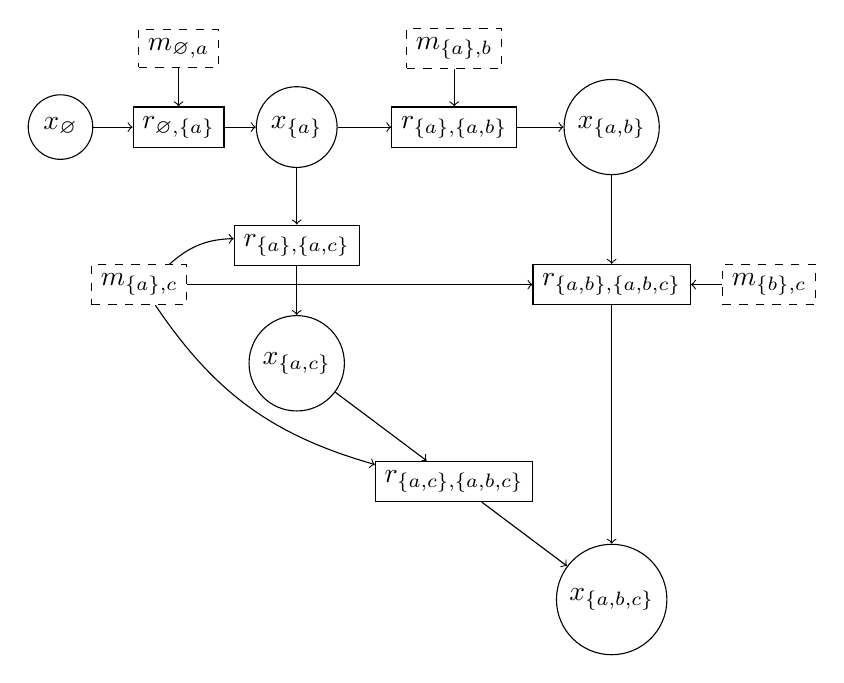
\begin{tikzpicture}
  \tikzset{
    _x/.style={circle,draw},
    r/.style={rectangle,draw},
    m/.style={rectangle,draw,dashed},
  };
  \node[_x] (_x-null) at (0,0)  {$x_{\varnothing}$};
  \node[_x] (_x-a)    at (3,0)  {$x_{\set{a}}$};
  \node[_x] (_x-ab)   at (7,0)  {$x_{\set{a,b}}$};
  \node[_x] (_x-ac)   at (3,-3) {$x_{\set{a,c}}$};
  \node[_x] (_x-abc)  at (7,-6) {$x_{\set{a,b,c}}$};

  \node[r] (r-null-a) at (1.5,0)  {$r_{\varnothing, \set{a}}$};
  \node[r] (r-a-ac)   at (3,-1.5) {$r_{\set{a}, \set{a,c}}$};
  \node[r] (r-a-ab)   at (5,0)    {$r_{\set{a}, \set{a,b}}$};
  \node[r] (r-ab-abc) at (7,-2)   {$r_{\set{a,b}, \set{a,b,c}}$};
  \node[r] (r-ac-abc) at (5,-4.5) {$r_{\set{a,c}, \set{a,b,c}}$};
  
  \node[m] (null-en-a) at (1.5, 1) {$m_{\varnothing, a}$};
  \node[m] (a-en-b)    at (5,1)    {$m_{\set{a}, b}$};
  \node[m] (a-en-c)    at (1,-2)   {$m_{\set{a}, c}$};
  \node[m] (b-en-c)    at (9,-2)   {$m_{\set{b}, c}$};

  \draw[->] (_x-null)      -- (r-null-a);
  \draw[->] (r-null-a)  -- (_x-a);
  \draw[->] (_x-a)         -- (r-a-ab);
  \draw[->] (r-a-ab)    -- (_x-ab);
  \draw[->] (_x-a)         -- (r-a-ac);
  \draw[->] (r-a-ac)    -- (_x-ac);
  \draw[->] (_x-ab)        -- (r-ab-abc);
  \draw[->] (r-ab-abc)  -- (_x-abc);
  \draw[->] (_x-ac)        -- (r-ac-abc);
  \draw[->] (r-ac-abc)  -- (_x-abc);
  \draw[->] (null-en-a) -- (r-null-a);
  \draw[->] (a-en-b)    -- (r-a-ab);
  \draw[->] (a-en-c)    -- (r-ab-abc);
  \draw[->] (b-en-c)    -- (r-ab-abc);
  \draw[->] (a-en-c) edge[bend left=20]  (r-a-ac);
  \draw[->] (a-en-c) edge[bend right=20] (r-ac-abc);
\end{tikzpicture}
\caption{Causal graph for Ex. \ref{ex:es}}
\label{fig:es-causal-graph}
\end{figure}

\end{exmp}

\begin{prop}
Given an event structure with $n$ events, constructing the
described causal graph requires $\mathcal{O}(2^n)$ operations.
\end{prop}
\section{Causal Model of Unsafe Behavior in Event Structure}

\subsection{Causal Model of Event Structure}
Let $\mathrm{E} = (E,\#,\vdash)$ be an event structure where
$E = \s{e_1, e_2, ...,e_n}$.
Let $S \subseteq \mc{P}(E)$ be the set of unsafe behaviors.
We define the causal model
$\mc{M} = (\mc{S},\mc{F},\mc{E})$ of unsafe behavior
in $\mr{E}$ where
$\mathcal{S} = (\mathcal{U},\mathcal{V},\mathcal{R})$.
We define $\mathcal{U}$ to be empty and $\mathcal{V}$
consisting of boolean variables as follows:
\begin{align*}
    \mathcal{V} = & \s{C_{e_i,e_j} ~|~  1 \leq i < j \leq n.
    e_i \in E \wedge e_j \in E}                                \\
                  & \cup \s{EN_{s,e} ~|~ s \in \mathcal{P}(E),
    e \in E. e \not \in s }                                    \\
                  & \cup \s{M_{s,e} ~|~ s \in \mathcal{P}(E),
        e \in E. e \not \in s }
\end{align*}
Intuitively, these variables model the existence of specific elements in
each of the event structure relations: $\#$, $\vdash_{min}$, and $\vdash$.
For two events $e,e' \in E$, variables of the form $C_{e,e'}$ represent whether $e\#e'$.
Similarly, for a subset of events $s \subseteq E$ and an event $e \in E$,
we use variables of the form $M_{s,e}$ and $EN_{s,e}$ to represent
whether $s \vdash_{min} e$ and $s \vdash e$ respectively.
Finally, we use a single boolean variable, $PV$, which denote the
violation of property in the event structure.
For each variable $X \in \mathcal{V}$ we define $\vec V_X$
as a vector of all variables in $\mathcal{V} \setminus \s{X}$.
For $x,y \in \mathcal{P}(E)$ we say $x$ is covered by $y$ written $ x \prec y$ iff:
\begin{align*}
    x \subseteq y \wedge x \neq y \wedge
    (\forall z. x \subseteq z \subseteq y \Rightarrow x = z
    \vee y = z)
\end{align*}
We define the functions in $\mathcal{F}$ as follows:
$$
    \f{C_{e,e'}} = \begin{cases}
        true  & \text{ if } e \# e' \\
        false & \text{ otherwise }
    \end{cases}
$$
$$
    \f{M_{s,e}} = \begin{cases}
        Min(s,e) \wedge Con(s) & \text{ if } s \vdash_{min} e \\
        false                  & \text{ otherwise }
    \end{cases}
$$
\begin{align*}
    \f{EN_{s,e}} & =
    \left(
    M_{s,e} \bigvee
    \left(
    \bigvee_{s'\prec s}EN_{s',e}
    \right)
    \right)
    \bigwedge
    Con(s)
\end{align*}
Where we have:
\begin{align*}
    Con(s)   & =   \left(
    \bigwedge_{ 1\leq j<j' \leq n \wedge e_j,e_{j'} \in s}
    \neg C_{e_j,e_{j'}}
    \right)               \\
    Min(s,e) & = \left(
    \bigwedge_{s' \subseteq E. (s' \subset s \vee s \subset s')
        \wedge e \notin s'}
    \neg M_{s',e}
    \right)
\end{align*}

\noindent Let $S \subseteq E$ be a subset of events.
We define $\varphi_S$, a boolean formula of primitive
events as follows:
\begin{align*}
    \left(
        \bigwedge_{\forall e,e' \in S} \neg C_{e,e'}
    \right)
    \bigwedge
    \left(
        \bigwedge_{\forall e \in S}
        \left(
            \bigvee_{\forall \pi \in \pi_S} 
            \left(
                EN_{\e,\pi_1} \wedge
                EN_{\s{\pi_1},\pi_2} \wedge
                \dots
                \wedge
                EN_{\s{\pi_1,...,\pi_{n_1}},p_n}
            \right)
        \right)
    \right)
\end{align*}

Where $\pi_S$ is the set of all permutations of $S$.
For a permutation $\pi \in \pi_S$, where $|S| = n$, 
we write $\pi_i$ where $1 \leq i \leq n$ for the $i$th 
element of $\pi$.

Thus, for a given subset of events $S \subseteq E$, 
we can use $\varphi_S$ as the effect for which we look
for a cause.


\subsection{Actual Cause of Unsafe Behavior}

Using the definition of the actual cause in the extended causal
model, we can rewrite the definition for unsafe behaviors in
event structures as follows:

\begin{definition}
    Let $\mr{E} = (E,\#,\vdash)$ be an event structure and
    $\mc{M}$ be the causal model of an unsafe behavior in
    $\mr{E}$ where unsafe behavior is specified as the
    function $F_{PV}$ in $\mc{M}$.
    We say $\vec X = \vec x$ is an actual cause of
    the unsafe behavior in $\mr{E}$ if the following
    conditions hold:
    \begin{itemize}
        \item  \textbf{AC1.} $M\models \vec X = \vec x
                  \wedge PV = \T$
        \item  \textbf{AC2. }There exists a partition $(\vec Z, \vec W)$ of $\mathcal{V}$ with $\vec X \subseteq \vec Z$ and some setting $(\vec x',\vec w')$ of the variables in $(\vec X,\vec W)$ such that if $(M,\vec u)\models \vec Z = z^*$ for all $Z\in \vec Z$, then both of the following conditions hold:

              (a) $M \models[\vec X \leftarrow \vec x', \vec W \leftarrow \vec w']
                  PV = \F
                  \wedge \vec V = \vec v
                  \wedge  \vec v \in \mathcal{E}$.

              (b) $M \models[\vec X\leftarrow \vec x, \vec W' \leftarrow \vec w', \vec Z'\leftarrow \vec z^*]
                  \vec V = \vec v
                  \wedge
                  (\vec v \in \mathcal{E} \Rightarrow PV = \T)
              $
              for all subsets $Z'$ of $\vec Z$.

        \item  \textbf{AC3.} $\vec X$ is minimal; no subset of $\vec X$ satisfies conditions $AC1$ and $AC2$.
    \end{itemize}
    Where $\vec v$ is the value of endogenous variables.
\end{definition}
\pagebreak


\section{Finding Root Causes for Unsafe Behavior}

\subsection{Minimal Enabling as a Cause}

\begin{thm}\label{thm:hp-x-y}
Given an event structure $\es$, a cause $X = S \vdash\,e$
where $(S, e) \in \vdash$, and an effect $Y = S_f$
where $S_f \in \conf{\es}$, $X$ is a cause of $Y$
(according to the HP definition) iff there is at least one path
from $m_{S,e}$ to $x_{S_f}$ in the causal graph of $\es$.
\end{thm}

\begin{proof}
We prove for both directions.

$\Leftarrow$: We check the conditions of HP causality for the given cause and effect.

\begin{itemize}
  \item \textbf{AC1:} Both the cause and effect hold in the factual scenario;
  therefore, this condition is satisfied.
\end{itemize}

For AC2.\{a,b\}, assume $(W, w, x')$ is the witness discussed by HP.

\begin{itemize}  
  \item \textbf{AC2.a:} The idea here is to restrict the causal graph
  such that the effect holds as long as the cause.
  
  Assume the path from cause to effect is as follows:
  \begin{equation}\label{eq:validating-path}
    m_{S,e} \rightarrow
    r_{S_1,S_2} \rightarrow
    x_{S_2} \rightarrow
    r_{S_2, S_3} \rightarrow
    \cdots \rightarrow
    r_{S_{k-1}, S_k} \rightarrow x_{S_k} = x_{S_f}
  \end{equation}

  We also define $W$ as:
  \[ \left( \In{r_{S_1, S_2}} \setminus \set{x_{S_1}, m_{S,e}} \right) \cup
    \left( \bigcup_{i=2}^k \In{x_{S_i}} \setminus \set{r_{S_{i-1}, S_i}} \right) \]
   
  The elements of $W$ are shown with dotted boxes in Fig. \ref{fig:witness}.
  All variables in $W$ are set to False ($w$ is an all-False valuation).
  $x'$ sets $r_{S,e}$ to False as well.
  
  \textbf{The choice of $W$ and validating path:}
  By defining $W$ as explained above, and setting it to all-False,
  the value for each vertex of the \textit{validating} path
  (as shown in Eq. \ref{eq:validating-path})
  can be determined by its predecessor. For $i \geq 2$, we have:
  \begin{equation}\label{eq:x-Si-restrict}
    (x_{S_i})_w = r_{S_{i-1}, S_i}
  \end{equation}
  
  By definition, each reason vertex consists of
  an \textit{enabling} and a \textit{configuration} component.
  We know the validating path is in the causal graph. Hence, for $i \geq 2$,
  the enabling component for $r_{S_i, S_{i+1}}$ is satisfied; so we have:
  \begin{equation}\label{eq:r-Si-Si+1-restrict}
    r_{S_i, S_{i+1}} = (r_{S_i, S_{i+1}})_w = x_{S_i} \wedge \text{True} = x_{S_i}
  \end{equation}
  
  For $r_{S_1,S_2}$, after setting $W$ to all-False, we have:
  \begin{equation}\label{eq:r-S1-S2-restrict}
    (r_{S_1,S_2})_w = \text{True} \wedge m_{S,e} = m_{S,e}
  \end{equation}
  
  \begin{figure}
\centering
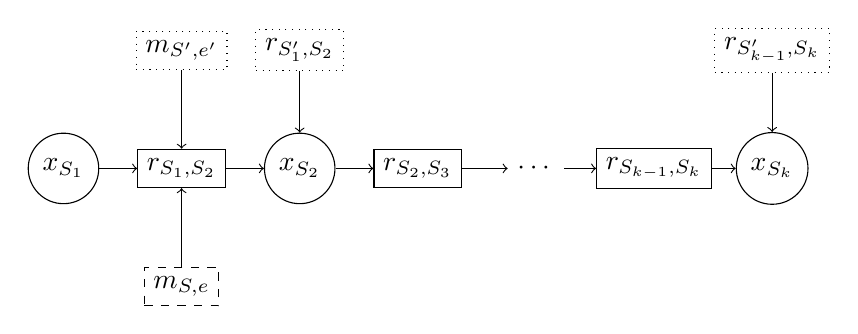
\begin{tikzpicture}
  \tikzset{
    _x/.style={circle,draw},
    r/.style={rectangle,draw},
    m/.style={rectangle,draw,dashed},
    w/.style={rectangle,draw,dotted},
  };
  \node[_x] (x-S1)       at (-1.5,0)  {$x_{S_1}$};
  \node[_x] (x-S2)       at (1.5,0)   {$x_{S_2}$};
  \node[_x] (x-Sk)       at (7.5,0)   {$x_{S_k}$};
  \node[m]  (m-S-e)      at (0,-1.5)  {$m_{S,e}$};
  \node[r]  (r-S1-S2)    at (0,0)     {$r_{S_1,S_2}$};
  \node[r]  (r-S2-S3)    at (3,0)     {$r_{S_2,S_3}$}; 
  \node[r]  (r-Sk-1-Sk)  at (6,0)     {$r_{S_{k-1},S_k}$};
  \node[w]  (m-S'-e')    at (0,1.5)   {$m_{S',e'}$};
  \node[w]  (r-S'1-S2)   at (1.5,1.5) {$r_{S'_1,S_2}$};
  \node[w]  (r-S'k-1-Sk) at (7.5,1.5) {$r_{S'_{k-1},S_k}$};
  \node     (dots)       at (4.5,0)   {$\cdots$};

  \draw[->] (x-S1)       -- (r-S1-S2);
  \draw[->] (m-S-e)      -- (r-S1-S2);
  \draw[->] (m-S'-e')    -- (r-S1-S2);
  \draw[->] (r-S1-S2)    -- (x-S2);
  \draw[->] (r-S'1-S2)   -- (x-S2);
  \draw[->] (x-S2)       -- (r-S2-S3);
  \draw[->] (r-S2-S3)    -- (dots);
  \draw[->] (dots)       -- (r-Sk-1-Sk);
  \draw[->] (r-Sk-1-Sk)  -- (x-Sk);
  \draw[->] (r-S'k-1-Sk) -- (x-Sk);
\end{tikzpicture}
\caption{Elements of $W$}
\label{fig:witness}
\end{figure}
    

  As shown in Eqs.
  \ref{eq:x-Si-restrict}, \ref{eq:r-Si-Si+1-restrict}, \ref{eq:r-S1-S2-restrict},
  Setting $m_{S,e}$ to False and $W$ to all-False will set all vertices
  in the validating path to False.

  With the witness described above, we can see that the effect $x_{S_f}$
  is also valuated as False; therefore, condition AC2.a is satisfied.
  
  
  \item \textbf{AC2.b:} After setting $m_{S,e}$ to True,
  while maintaining $W$ as all-False, $x_{S_f}$ is valuated to True again;
  this follows from the equations of the validating path when $W$ is set to all-False.
  The \textit{validating edges} for $x_{S_f}$ are shown with thick lines
  in Fig. \ref{fig:ac2.b}. Observe that, re-setting any variable $v \not\in W$
  does \textbf{not} \textit{invalidate} the specified path for $x_{S_f}$.

  \input{./fig/fig:ac2.b}

  \item \textbf{AC3:} As our cause is a singleton,
  this condition is also satisfied.
\end{itemize}

$\Rightarrow$: Assume there is no path from $m_{S,e}$ to $x_{S_f}$
in the causal graph. The vertices remaining after a W-projection will be
$m_{S,e}$, $x_{S_f}$, and all parent vertices of $x_{S_f}$ (unreachable from $m_{S,e}$).
Assume we have chosen $(W, w, x')$ such that AC2.a is satisfied
(i.e. $Y_{wx'} = \text{False}$).
As there is no path from $m_{S,e}$ to $x_{S,f}$, we have: $Y_{wx} = Y_{w} = \text{False}$.
Hence, AC2.b cannot be satified, for any arbitrary $W$, which contradicts our assumption
$m_{S,e} \propto x_{S_f}$.

\end{proof}

\begin{thm}\label{thm:hp-x-disj-Y}
Given an event structure $\es$, a cause $X = S \minen e$,
and an effect $Y = \bigvee_{f} S_{f}$
where $\forall f.\;S_f \in \conf{\es}$, $X$ is a cause of $Y$
(according to the HP definition) iff there exists $f$ such that
there is at least one path from $m_{S,e}$ to $x_{S_f}$
in the causal graph of $\es$.
\end{thm}

\begin{proof}
We prove for both directions.

$\Leftarrow$: Assume there is a path from $m_{S,e}$ to $x_{S_f}$ for some $f$.
Also assume $W$ is defined as in Thm. \ref{thm:hp-x-y}. For this problem,
we construct the new witness $W'$ as follows:
\[ W' = W \cup \left( \bigcup_{f' \neq f} x_{S_{f'}} \right) \]

$W'$ is set to all-False, as before.

With the new witness, AC2.\{a,b\} can be satisfied
for the new problem.

$\Rightarrow$: Using an argument similar to the proof for Thm. \ref{thm:hp-x-y},
we can show that if $x \propto y$, there is at least one path from $m_{S,e}$ to $x_{S_f}$ for some $f$.
\end{proof}

\begin{thm}\label{thm:hp-x-conj-Y}
Given an event structure $\es$, a cause $X = S \minen e$,
and an effect $Y = \bigwedge_{f} S_{f}$ where $\forall f.\;S_f \in \conf{\es}$,
$X$ is a cause of $Y$ (according to the HP definition)
iff there exists $f$ such that there is at least one path from $m_{S,e}$ to $x_{S_f}$
in the causal graph of $\es$.
\end{thm}

\begin{proof}
$\Leftarrow$: The set $W$ is selected just as done in Thm. \ref{thm:hp-x-disj-Y}.
For any $w \in W \cap Y$, we set $w$ to True.

$\Rightarrow$: Similar to Thms. \ref{thm:hp-x-y}, \ref{thm:hp-x-disj-Y}.
\end{proof}

% \subsection{False Minimal Enabling as a Cause}

% In the previous section, we showed how to check causality for
% true minimal enabling relations
% (i.e. $S \vdash e =$ True in the given event structure).
% Now we want to improve the existing causal graph
% to include false minimal enabling relations as well.

% Given event structure $\es = (E, \#, \vdash)$,
% For each $S \subseteq E$ and $e \in E$, we define vertex $r_{S,e}$.
% The value associated with this vertex will be as follows:

% \[ m_{S,e} =
%   \begin{cases}
%     \Min{S}{e}   & \text{if } S \vdash_{min} e \\
%     \text{False} & \text{otherwise}
%   \end{cases}
% \]

% Where $\Min{S}{e}$ is defined as follows:
% \[ \Min{S}{e} =
%   \bigwedge_{S' \subseteq E.\;(S' \subset S) \vee (S \subset S')}
%   \neg m_{S',e}
% \]

% Informally, if $S$ minimally enables $e$, no pure sub- or super-set of $S$
% minimally enables $e$.

\subsection{False Conflict as a Cause}

As we construct the configurations lattice for an event structure, we check for both
conflicts and enablings. The causal graph described before only contains the enabling
steps. We can refine the previous model to account for conflicts as well.

\subsubsection{Causal Graph}

We add new vertices $c_{e,e'}$ to the graph previously described, where
$c_{e,e'}$ shows the conflict between the events $e, e'$.
For any edge $x_S \rightarrow r_{S,S'}$, we remove this edge,
add the new vertex $r^{(c)}_{S,S'}$, and add edges $x_S \rightarrow r^{(c)}_{S,S'}$ and
$r^{(1)}_{S,S'} \rightarrow r_{S,S'}$. We also re-label all previous $r$-vertices to $r^{(m)}$-vertices.
For each vertex $r^{(c)}_{S,S'}$, we add edges $c_{f,e} \rightarrow r^{(c)}_{S,S'}$,
where $e = S' \setminus S$ and $f \in S$.

\subsubsection{Causal Model}

All $m$- and $x$-variables are defined exactly as before.
We only re-define $r$-variables, and define $c$-variables.

\begin{itemize}
  \item $r^{(c)}_{S,S'}$ ($S,S' \subseteq E$): We have:
  \[ r^{(c)}_{S,S'} = x_S \wedge
    \left( \bigwedge_{ c_{f,e} \in \In{ r^{(c)}_{S,S'} } } \neg c_{f,e} \right) \]
  
  Informally, a reason variable $r^{(c)}_{S,S'}$ checks the conflict part for
  the induction step for obtaining configuration $S'$ from $S$.
  \item $r^{(c)}_{S,S'}$ ($S,S' \subseteq E$): We have:
  \[ r^{(m)}_{S,S'} = r^{(c)}_{S,S'} \wedge
    \left( \bigvee_{ m_{S,e} \in \In{ r^{(m)}_{S,S'} } } m_{S,e} \right) \]
  
  Informally, a reason variable $r^{(m)}_{S,S'}$ checks the enabling part for
  the induction step for obtaining configuration $S'$ from $S$.
  \item $c_{e,f}$ ($e,f \in E$): These variables hold the constant value of True.
  To avoid duplication, we only define one $c$-variable (and $c$-vertex) for a given pair $e,f$.
\end{itemize}

\subsubsection{Causality}

With the refined causal model, we can easily show
Thms. \ref{thm:hp-x-y}, \ref{thm:hp-x-disj-Y}, \ref{thm:hp-x-conj-Y} hold
when cause is a false conflict instead of a true minimal enabling relation.

% \begin{thm}\label{thm:hp:c:x-y}

% \end{thm}

\end{document}